\documentclass[10pt,a4paper]{article}
\usepackage[margin=1.9cm]{geometry}
\usepackage[T1]{fontenc}
\usepackage[utf8]{inputenc}
\usepackage{lmodern}
\usepackage{amsmath,amssymb}
\usepackage{graphicx}
\usepackage{booktabs}
\usepackage[numbers,sort&compress]{natbib}
\usepackage{xcolor}
\usepackage[colorlinks=true,linkcolor=black,citecolor=black,urlcolor=blue]{hyperref}
% Compact lists and small captions without extra packages (TinyTeX/Overleaf-safe).
\let\olditemize\itemize
\renewcommand{\itemize}{\olditemize\setlength{\itemsep}{1pt}\setlength{\parskip}{0pt}\setlength{\topsep}{2pt}}
\makeatletter\renewcommand{\@makecaption}[2]{\vskip 4pt{\small\textbf{#1.} #2\par}}\makeatother
\setlength{\parskip}{3pt}
\setlength{\parindent}{0pt}
\newcommand{\dec}{\,dec}            % decades of log10 f
\newcommand{\ci}[2]{[#1,\,#2]}      % 95% bootstrap interval
\newcommand{\todo}[1]{\textcolor{red}{\textbf{[TODO: #1]}}}

\title{\vspace{-1.2cm}Can the search tilt? Geometry as an explanation for\\
Bayesian optimisation versus CMA-ES\vspace{-0.3cm}}
\author{\todo{Name 1 (student number)}, \todo{Name 2 (student number)}, \ldots\\[2pt]
\small Repository: \todo{\url{https://github.com/USER/REPO}}}
\date{\vspace{-0.6cm}}

\begin{document}
\maketitle

\begin{abstract}
\noindent
We test one explanation for a difference between Bayesian optimisation (BO) and CMA-ES: on a rotated,
ill-conditioned problem, what matters is whether a method's search geometry can tilt away from the
coordinate axes, not which family it belongs to. We run a $2\times2$ ablation: full against diagonal
covariance for CMA-ES, and a full kernel metric against the standard ARD kernel for BO. Diagonal CMA-ES
fails only when the valley lies between the axes. ARD cannot even represent the tilt. A first
head-to-head showed \emph{no} rotation penalty for BO. We traced that negative result to a fitting failure
that made BO stall on every problem. Once it was fixed, BO-ARD paid a rotation penalty of $+2.0$ decades
at $\kappa=10^4$ while the full metric did not, the same pattern as diagonal against full CMA-ES. We then
test which of CMA-ES's theoretical invariances survive in practice (rank invariance does, bit for bit;
units invariance only with a matched initial covariance) and where the box boundary, a curved valley and
noise change the comparison. Under noise, the rule for choosing the final point mattered as much as how
the budget was split. With each family's best choices the two are level. Nothing here is specific to one family: the axis restriction, not the
algorithm, predicts the rotation failures.
\end{abstract}

%=====================================================================
\section{Question and explanation under test}
%=====================================================================
CMA-ES adapts a full covariance matrix from the ranking of sampled candidates, so its sampling
distribution can stretch and \emph{rotate} to match the local Hessian \citep{hansen2016tutorial}. BO fits
a Gaussian-process surrogate and chooses points through an acquisition function \citep{frazier2018tutorial}.
Its standard squared-exponential kernel with automatic relevance determination (ARD) uses a squared
distance $\sum_i (x_i-x'_i)^2/\ell_i^2$, a \emph{diagonal} metric. Trust-region BO inherits the same
restriction, because TuRBO's trust region is a hyperrectangle whose side lengths are set per coordinate
from the ARD lengthscales \citep{eriksson2019turbo} (tested in Section~4).

\textbf{Explanation under test.} On a rotated, ill-conditioned problem, performance depends on whether
the method's search geometry \emph{can tilt}. That property, not the family, decides the outcome:
\begin{itemize}
\item \emph{can tilt:} full-covariance CMA-ES, and a GP with a full metric $M=LL^\top$ in
$k(x,x')=\exp(-\tfrac12(x-x')^\top M(x-x'))$;
\item \emph{cannot tilt:} diagonal CMA-ES, and the ARD kernel ($M$ diagonal).
\end{itemize}
\textbf{Conditioning, rotation and curvature.} Near a minimum, $f(x^*+h)\approx f^*+\tfrac12 h^\top Hh$.
The eigenvalues of the Hessian $H$ are the \emph{curvatures} of $f$ along its eigenvectors. The
\emph{condition number} $\kappa=\lambda_{\max}/\lambda_{\min}$ is the ratio of the largest curvature to the
smallest, so an ill-conditioned problem is a narrow valley: steep across, flat along. The eigenvectors
give the valley's \emph{orientation}; a rotation changes them but leaves $\kappa$ unchanged. This is why
our problems vary $\kappa$ and rotation separately. On a quadratic, $H$ is the same everywhere, so one
tilt describes the whole problem. A well-adapted CMA-ES covariance approximates $H^{-1}$ up to scale
\citep{hansen2016tutorial}, and a full GP metric can align with the eigenvectors of $H$. A step that
ignores the orientation is a poor one on a narrow, tilted valley. Along the valley it must stay short
enough not to climb the steep walls, so progress along the flat direction is slow. Rosenbrock
(Section~\ref{sec:beyond}) adds a third property: its Hessian changes from point to point. The valley
floor \emph{bends}, so the local orientation and local $\kappa$ change along the path. This separates
\emph{local} geometry, which CMA-ES re-adapts as it moves, from \emph{global} geometry, the single metric a
stationary kernel learns for the whole box.

The explanation makes three falsifiable predictions. (i) Each axis-restricted method pays a penalty
under rotation that its tilting counterpart does not. (ii) The penalty appears only when the problem is
both ill-conditioned and rotated, because an aligned problem needs no tilt. (iii) The tilting variant
pays a modest price when no tilt is needed, because it has more parameters to learn. A brief
from the course also asks which theoretical invariances survive the implementation, and how changes of units and
box constraints behave; Sections~\ref{sec:invariance}--\ref{sec:beyond} take these up.

%=====================================================================
\section{Methods and experimental design}
%=====================================================================
\textbf{Problems.} Ellipsoids $f(x)=\tfrac12(x-x^*)^\top QDQ^\top(x-x^*)$ with log-spaced eigenvalues
from 1 to $\kappa$, following COCO practice \citep{hansen2021coco}: the optimum $x^*$ is drawn on a
radius-2 sphere (never at the start point), $Q$ is the identity (aligned), a fixed angle, or a Haar-random
rotation, and each \emph{instance} fixes $Q$ and $x^*$ from its index. Section~\ref{sec:beyond} adds
Rosenbrock (COCO f8/f9 \citep{hansen2009bbobfunctions}) and additive Gaussian noise.

\textbf{Methods.} CMA-ES follows Hansen's tutorial (rank-one and rank-$\mu$ updates, cumulative step-size
adaptation, default population; $\lambda=6$ in 2-D). The diagonal variant zeroes the off-diagonal
covariance entries after every update. BO is GP-EI: an initial uniform design of $2d+4$ points, EI
maximised over 200 uniform candidates and then polished with L-BFGS-B inside the box. Targets are
log-transformed and standardised before fitting. GP hyperparameters are fitted by MAP with BoTorch's
dimension-scaled LogNormal lengthscale prior \citep{hvarfner2024vanilla}, with 10 restarts and exact
marginal-likelihood gradients \citep[eq.~5.9]{rasmussen2006gpml}. We place the prior on the
\emph{eigen}-lengthscales of $M$, so that it does not favour axis-aligned metrics, which would build in
the restriction under test. All four methods are implemented in NumPy/SciPy in the repository, so every
kernel and update choice is visible.

\textbf{Budget rule (shared by E2--E5).} Cost is counted in objective evaluations, by wrapping the
objective; the initial design counts. Both families get the same box $[-5,5]^d$: BO searches it, and
CMA-ES starts at its centre with $\sigma_0=0.3\times$ box width and is not otherwise constrained (the
asymmetry is examined in Section~\ref{sec:boundary}). The cap is 200 evaluations. Every evaluation is
logged, so each run gives both a fixed-budget view ($f_{\text{best}}$ at 20/50/100/200) and runtimes to
targets $10^{-1},10^{-3},10^{-5}$, with failures reported as success rates rather than dropped
\citep{hansen2021coco}. Wall-clock time is logged because it separates the families sharply (about
0.002\,s per CMA-ES run against 120--260\,s per BO run). Instance index = seed for every method, so
cross-method comparisons are paired; we report median differences in $\log_{10} f$ (``decades'') with 95\%
bootstrap intervals over 15 instances. Aligned-against-rotated comparisons are unpaired, because the
rotation is drawn together with the optimum.

\textbf{Reproducibility.} Each experiment is one script in \texttt{code/} that writes CSVs to
\texttt{results/}. Section 8 of the notebook reloads every number quoted here, and
\texttt{code/make\_figures.py} rebuilds every figure from the CSVs. BO runs are bit-reproducible when
BLAS is single-threaded, which the scripts enforce. With multithreaded BLAS, two runs of one seed
differed by $6\times10^{-5}$ in relative terms, and the difference compounds; results are reproducible
in distribution across machines, not run for run (details in \texttt{readme.md}).

%=====================================================================
\section{The tilt in each family}
%=====================================================================
\textbf{E1: CMA-ES.} At $\kappa=1{,}000$ in 2-D (15 instances, 4,000 evaluations, target $10^{-8}$),
diagonal CMA-ES solves every instance at $0^\circ$ and $90^\circ$ and none between $30^\circ$ and
$60^\circ$; full CMA-ES solves every angle (Fig.~\ref{fig:e1}). The $90^\circ$ point is the control: it
only swaps the axes, so recovery there shows that the rotation, not the conditioning, causes the
failure. At $\kappa=100$ both variants succeed at every angle, as prediction (ii) requires. Under
Haar-random rotation full CMA-ES needs 405 against 408 median evaluations (30 instances), the rotation
invariance claimed by \citet{hansen2016tutorial}, while diagonal success drops to 47\%, and to 0\% by
$d=16$. On aligned problems the full variant costs up to 21.6\% more evaluations at $d=32$, because it
learns $d(d+1)/2$ covariance entries instead of $d$: prediction (iii).

\begin{figure}[t]
\centering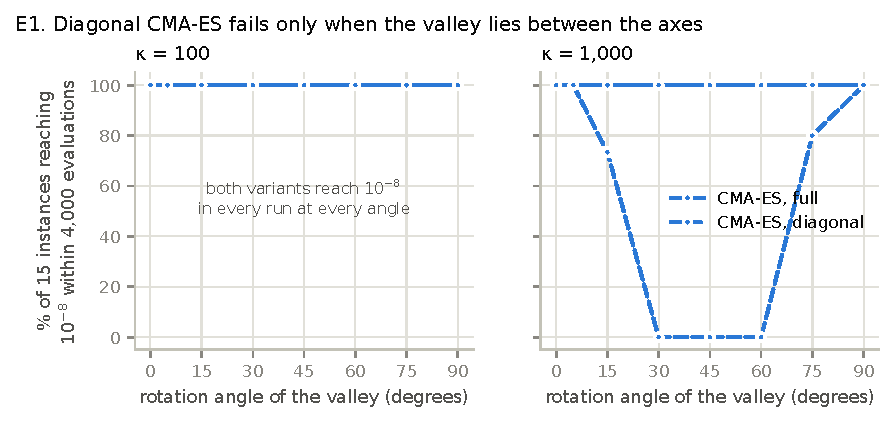
\includegraphics[width=0.86\linewidth]{figures/fig1_e1_angle_sweep.pdf}
\caption{E1. Success of full (solid) and diagonal (dashed) CMA-ES against the angle of a 2-D valley.}
\label{fig:e1}
\end{figure}

\textbf{E2c: the surrogate.} Rather than infer the kernel's geometry from optimisation performance, we
read it directly. We fit both kernels to the same 40-point uniform designs (10 instances) and measure
the angle between the learned long axis and the true flat direction (Fig.~\ref{fig:e2c}). ARD is off by
exactly $45^\circ$ on $45^\circ$ problems at every $\kappa$, and by a median $18.1^\circ$ under random
rotation; the full metric is within $0.2^\circ$--$4.1^\circ$. On rotated problems ARD's held-out RMSE is
1.3--1.9$\times$ the full metric's from $\kappa=100$. On aligned ones ARD is better (ratio 0.75--0.93 at
$\kappa=10$--1,000), the surrogate-side counterpart of the CMA-ES overhead.

An earlier maximum-likelihood fit had a hidden bound $\ell\le e^4$: the long lengthscale sat on it in
60--80\% of fits at $\kappa\ge10^3$ (E2d), so any lengthscale \emph{ratio} we reported was set by the
bound, not by the data. The MAP prior removed every bound hit and left the axis errors unchanged. We
therefore report direction and RMSE, not ratios.

\begin{figure}[t]
\centering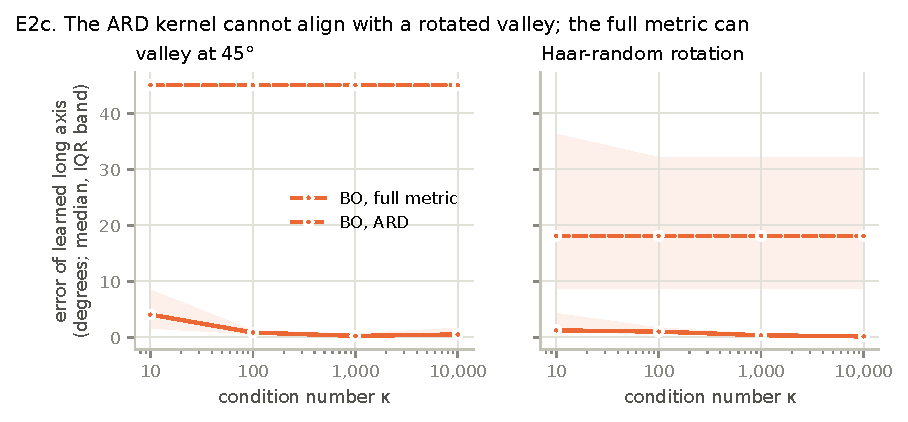
\includegraphics[width=0.86\linewidth]{figures/fig2_e2c_axis_error.pdf}
\caption{E2c. Error of the GP's learned long axis (median over 10 instances; band = interquartile range).}
\label{fig:e2c}
\end{figure}

%=====================================================================
\section{Head to head, a negative result, and its cause}
%=====================================================================
\textbf{E2, first run.} Under the budget rule (2-D; $\kappa\in\{1,100,10^4\}$; aligned and random
rotation; 15 instances), BO led CMA-ES by 0.6--1.0\dec{} at 20 evaluations, and CMA-ES led by
2.3--3.8\dec{} at 200 for $\kappa\le100$. On rotation, however, prediction (i) \emph{failed} for BO: BO-ARD's
rotation penalty at $\kappa=100$ was $+0.05$ \ci{-0.53}{+0.63} decades, while diagonal CMA-ES paid
$+1.70$ \ci{+0.41}{+2.57}. A second anomaly stood out: BO stalled near $10^{-2.6}$ even on the round bowl
($\kappa=1$), the easiest case for a GP, and no BO run reached $10^{-5}$.

\textbf{E2e, diagnosing the stall.} We re-ran BO on the round bowl with per-iteration logging, behaviour
unchanged, and tested four hypotheses, each with its own signature:
\begin{itemize}
\item \emph{Floor in the log transform:} rejected. The best value stayed 54--82$\times$ above it.
\item \emph{The acquisition search misses the improving region:} rejected. A dense search around the
incumbent found no more EI than the random candidates did.
\item \emph{EI underflow:} the mechanism. After 50 evaluations the largest EI anywhere was below
$10^{-12}$ in 97--100\% of iterations. The chosen points landed a median 3.8 from the incumbent in a box
of width 10, so BO was effectively sampling at random.
\item \emph{The GP explains the optimum away as noise:} the cause. The fitted noise SD was 0.2--0.4
(standardised units) on a noise-free objective. The posterior mean at the incumbent sat about 1.5 units
above its observed value, 2--2.5$\times$ the gap to the second-best point. EI, measured against an
incumbent the model considers unreachable, collapses.
\end{itemize}
Changing one thing at a time (BO-ARD, same instances, paired), fixing the noise variance at $10^{-6}$
improved the median by $-1.43$ \ci{-1.83}{-0.73} decades at 50 evaluations and $-1.17$ \ci{-1.71}{-0.74}
at 200; every run then reached $10^{-3}$ (27\% before). LogEI \citep{ament2023logei}, which fixes the
underflow but not its cause, changed nothing ($+0.01$ \ci{-0.79}{+0.47}). Lowering the transform floor as
well added a non-significant $-0.28$ \ci{-0.68}{+0.15}, so we adopted the fixed noise alone. Even fixed,
BO stops improving near $10^{-4}$. The fixed-noise logs explain why: the acquisition search now fails,
the hypothesis rejected before the fix. After 100 evaluations the GP's shortest lengthscale is about
0.07, so the region worth searching is about 0.1 wide. In 98--99\% of iterations a dense search there
finds $>10\times$ (median about $800\times$) the EI of the point chosen, while only 1--2\% of chosen
points land within 0.1 of the incumbent: 200 uniform candidates in a $10\times10$ box almost never hit it.
Adding 200 candidates around the incumbent, as BoTorch samples around its best points, removed the
stall on the round bowl: every run reached $10^{-5}$, in a median of 41--56 evaluations against about 145
for CMA-ES. It also exposed a \emph{boundary trap}. On the ill-conditioned problems, 4--8 of 15 runs per
aligned cell ended at $f\approx5$, with the incumbent on the valley floor \emph{at the box edge} and
95--96\% of evaluations on the edge. EI's boundary preference (Section~\ref{sec:boundary}) places the
incumbent there, and searching around it keeps BO there.

\textbf{E2 with the fix.} We re-ran the 180 BO runs both ways on one machine, fitted noise and fixed
noise (CMA-ES is unaffected), so the comparison is paired. The fix lifted BO significantly in 10 of 12
condition, geometry and kernel cells, by 0.68--1.50 decades at 200 evaluations. \textbf{The negative
result reversed} (Fig.~\ref{fig:pen}). With fitted noise, neither kernel showed a rotation penalty on
this machine either (BO-ARD at $\kappa=10^4$: $+0.04$ \ci{-0.27}{+0.71}). BO-ARD's rotation penalty became $+0.54$ \ci{+0.24}{+1.41}
decades at $\kappa=100$ and $+2.01$ \ci{+1.28}{+2.97} at $\kappa=10^4$; BO-full's stayed non-significant
($+0.24$ \ci{-0.43}{+1.13}, $+0.49$ \ci{-0.03}{+0.66}). Paired on the same rotated $\kappa=10^4$
instances, BO-ARD ended 1.40 \ci{+0.68}{+1.69} decades behind BO-full; on aligned ones the two were level
($-0.13$ \ci{-1.15}{+0.19}). This is the CMA-ES pattern in a different family: the stall had been hiding
the ARD penalty, because no method can lose ground it never gains.

Across families (Fig.~\ref{fig:curves}), BO-full now leads CMA-ES-full by 0.85--1.25 decades at 50
evaluations in every cell, and on aligned $\kappa=10^4$ at every budget ($-1.32$ \ci{-1.92}{-0.62} at 200).
With plain EI, CMA-ES still wins by 200 evaluations at $\kappa\le100$ (by 1.2--2.7 decades), where its
linear convergence overtakes BO's stalled progress. That conclusion depends on the acquisition search.
A TuRBO-style trust-region BO (below) beats full CMA-ES at 200 evaluations on aligned $\kappa=100$ ($-1.36$
\ci{-2.02}{-0.85}) and on rotated $\kappa=10^4$ ($-3.32$ \ci{-4.24}{-1.82}). BO's early lead costs about
$10^5$ times more computation per run (trust-region BO: 41--79\,s per run).

\textbf{Robustness of the rotation result.} The ARD penalty could be an artefact of one kernel or one
acquisition search, so we repeated the key comparison with three changes (Table~\ref{tab:robust}): BoTorch's
default Mat\'ern-5/2 kernel (E8); 200 extra candidates around the incumbent; and a TuRBO-style trust
region (E10; one region, TuRBO-1's expand/shrink/restart rules, EI over 1,000 candidates inside it). The
trust region is either the published axis-aligned box with sides scaled by the ARD lengthscales, or a
box rotated to the full metric. In all four variants the axis-restricted version ends significantly
behind on rotated $\kappa=10^4$ problems and is level on aligned ones. This confirms the argument of
Section~1 that TuRBO inherits the restriction. On aligned $\kappa=100$ the axis-aligned trust region is
\emph{better} ($-0.57$ \ci{-1.04}{-0.27}): the cost of tilting when no tilt is needed, again.

\begin{table}[t]
\centering\small
\begin{tabular}{lcc}
\toprule
BO variant (2-D, 15 instances, 200 evaluations) & rotated $\kappa=10^4$ & aligned $\kappa=10^4$ \\
\midrule
EI, squared exponential (E2, fixed noise) & $+1.40$ \ci{+0.68}{+1.69} & $-0.13$ \ci{-1.15}{+0.19} \\
EI, Mat\'ern-5/2 (E8) & $+1.06$ \ci{+0.59}{+1.43} & $-0.13$ \ci{-0.70}{+0.54} \\
EI + local candidates & $+1.28$ \ci{+0.12}{+2.36} & $-2.96$ \ci{-3.44}{+2.61} \\
Trust region, ARD box vs rotated box (E10) & $+2.92$ \ci{+1.27}{+3.79} & $-0.39$ \ci{-3.11}{+4.65} \\
\bottomrule
\end{tabular}
\caption{Axis-restricted minus tilting version, median $\log_{10}f$ at 200 evaluations, paired by instance
(+ = axis-restricted worse). The wide aligned intervals in the last two rows come from the boundary trap.}
\label{tab:robust}
\end{table}

\begin{figure}[t]
\centering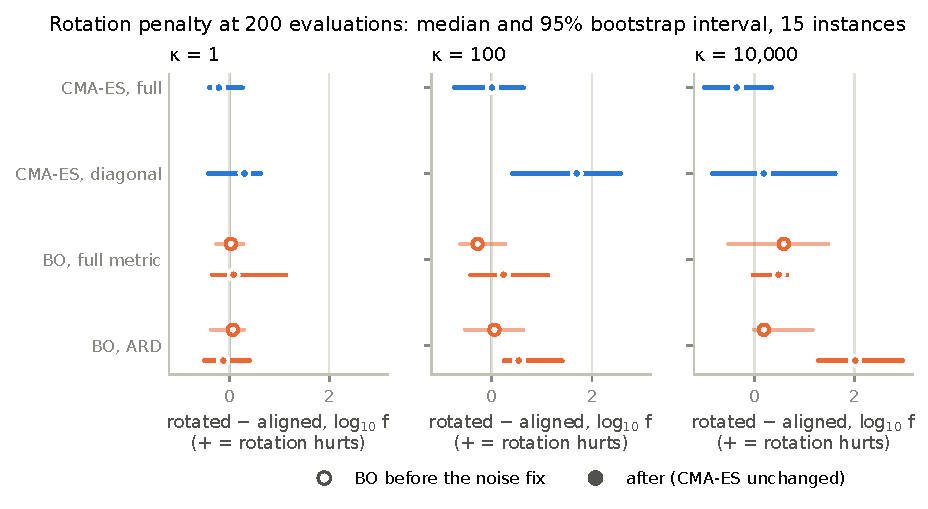
\includegraphics[width=0.86\linewidth]{figures/fig4_rotation_penalty.pdf}
\caption{Rotation penalty at 200 evaluations (median and 95\% bootstrap interval). Hollow: BO before the
noise fix (same machine, paired instances). The axis-restricted variant pays in both families once BO is no longer stalled.}
\label{fig:pen}
\end{figure}

\begin{figure}[t]
\centering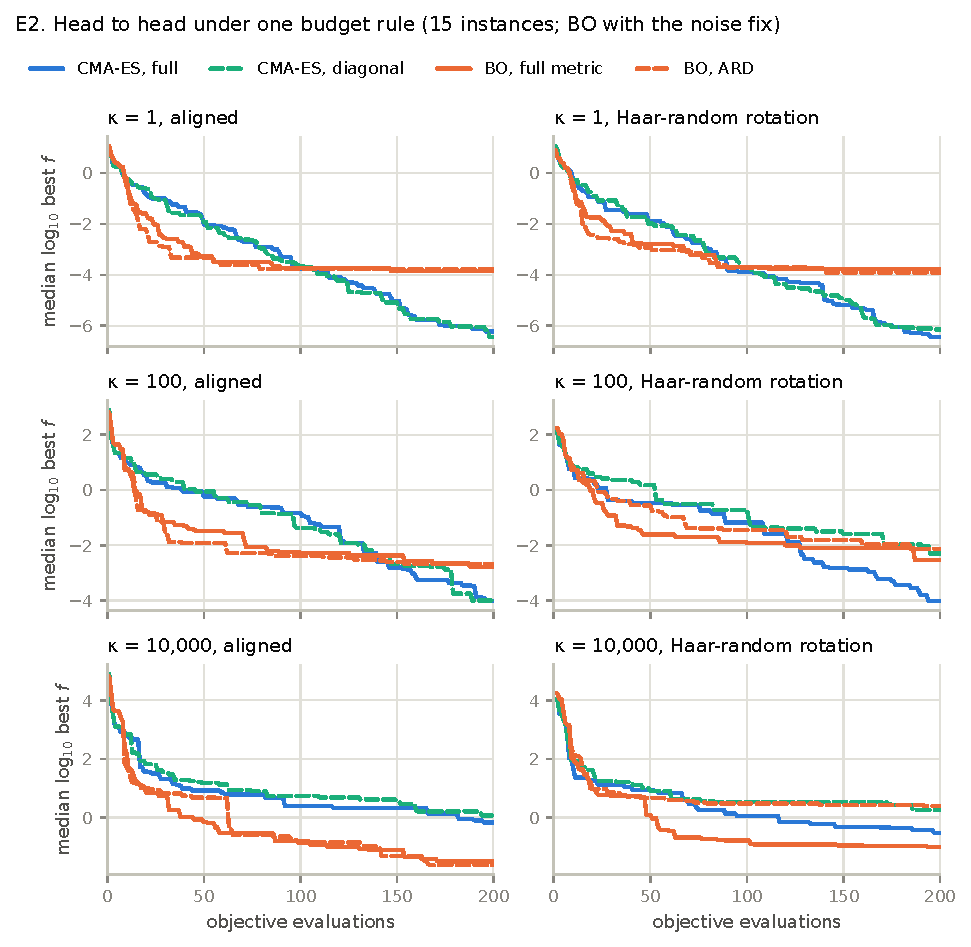
\includegraphics[width=0.80\linewidth]{figures/fig3_e2_curves.pdf}
\caption{E2 with the BO fix: median best-so-far over 15 instances. Colour = family; dashed = axis-restricted.}
\label{fig:curves}
\end{figure}

%=====================================================================
\section{Which invariances survive the implementation?}\label{sec:invariance}
%=====================================================================
\textbf{E3} (Fig.~\ref{fig:e3}; aligned $\kappa=100$; paired with an untransformed baseline; every
evaluation scored on the original $f$). Hansen lists invariance to strictly increasing transformations
of $f$, and to invertible linear maps of the search space \emph{provided the initial mean and covariance
are mapped with it} \citep{hansen2016tutorial}.
\begin{itemize}
\item \emph{Monotone maps of $f$} (log1p, cube, square root, $f+1$). Both CMA-ES variants produced runs
bit-identical to the baseline in all 120 cases. BO is not invariant, and the direction depends on the
map. Cubing costs $+1.72$ \ci{+1.14}{+2.22} (ARD) and $+1.74$ decades (full), and no run reaches
$10^{-3}$; log1p helps BO-full ($-0.52$ \ci{-0.98}{-0.03}). The cube result has a precise cause in our
implementation: the target floor is $10^{-6}\times$ the spread of observed values, and cubing stretches
the spread so much that the floor corresponds to $f\approx14$, below which BO sees nothing. The floor is
not the whole story, though: square root makes it far finer ($10^{-9}$) without helping.
\item \emph{Units} ($u_i=x_i/s_i$). With default set-ups, no method is invariant: $s=(1,10)$ raises the
effective conditioning to $10^4$ and costs CMA-ES about $+3.9$ decades and BO $+1.3$--1.4. Mapping
CMA-ES's initial covariance as the theory requires ($C_0=S^{-2}$) restores invariance: exactly (to
$10^{-12}$) for the diagonal variant, and in distribution for the full one ($+0.21$ \ci{-1.07}{+0.85}).
The full variant is not identical run for run, because its eigendecomposition sorts the axes by
eigenvalue and so reassigns the random draws. BO's equivalent, normalising each input to its own range
\citep{balandat2020botorch}, is invariant by construction, but our box has one width for all coordinates,
so it was not run.
\end{itemize}

\begin{figure}[t]
\centering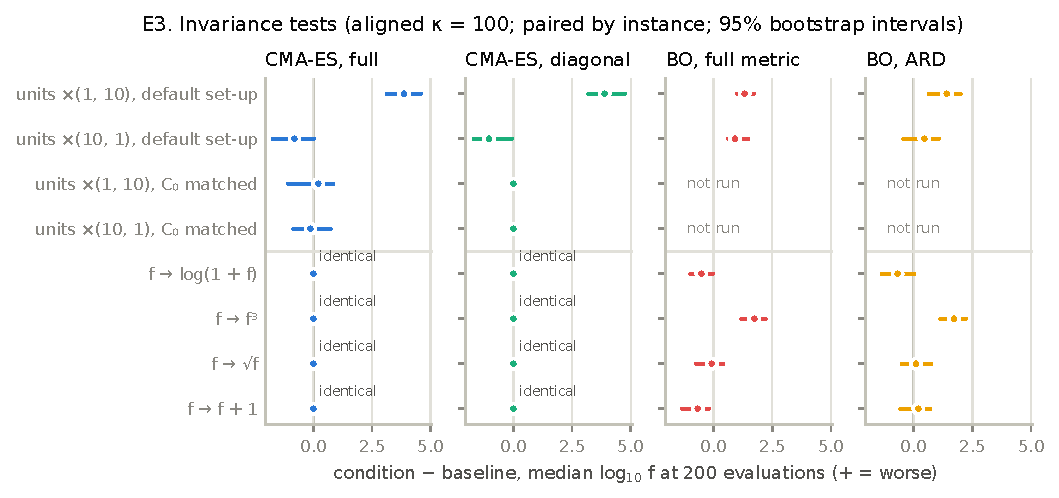
\includegraphics[width=0.92\linewidth]{figures/fig5_e3_invariance.pdf}
\caption{E3. Condition minus baseline, median $\log_{10}f$ at 200 evaluations (+ = worse); ``identical'' =
all 15 runs bit-identical to the baseline.}
\label{fig:e3}
\end{figure}

%=====================================================================
\section{The box boundary}\label{sec:boundary}
%=====================================================================
\textbf{E4} (Fig.~\ref{fig:e4}; 2-D aligned, $\kappa\in\{1,100\}$). Because every method starts at the
centre, an optimum near an edge is also far from the start. We therefore compare each edge position with
an interior control at the same distance ($(\pm3.5,\pm3.5)$, 1.5 from both faces).
\begin{itemize}
\item \emph{BO} is worse when the optimum lies 0.1 inside the edge ($+1.62$ \ci{+0.57}{+2.10} at
$\kappa=1$, $+0.73$ \ci{+0.31}{+0.99} at $\kappa=100$) and better when it lies exactly on it ($-0.95$,
$-1.68$, both significant). BO puts 9--15\% of its evaluations exactly on the boundary, consistent with
GP-EI's known over-exploration there \citep{siivola2018boundary}: the posterior variance is largest where
there is no data beyond the edge, and the bounded EI optimiser stops exactly on it. With the optimum in a
corner, BO evaluates it exactly in 93--100\% of runs, at a median of evaluation 9--10. That is an artefact
of this preference, not evidence of better search.
\item \emph{Unconstrained CMA-ES} stays within 0.53 decades of the control everywhere; it is affected by
distance from the start, not by the edge. But 47--63\% of its evaluations fall outside the box when the
optimum is on an edge or in a corner. A reflection boundary transform (a simplified version of pycma's
default) removes the violations at no significant cost, except when its periodicity lets the mean
drift onto a mirror copy of an interior optimum ($+1.04$ \ci{+0.43}{+1.64}).
\end{itemize}

\begin{figure}[t]
\centering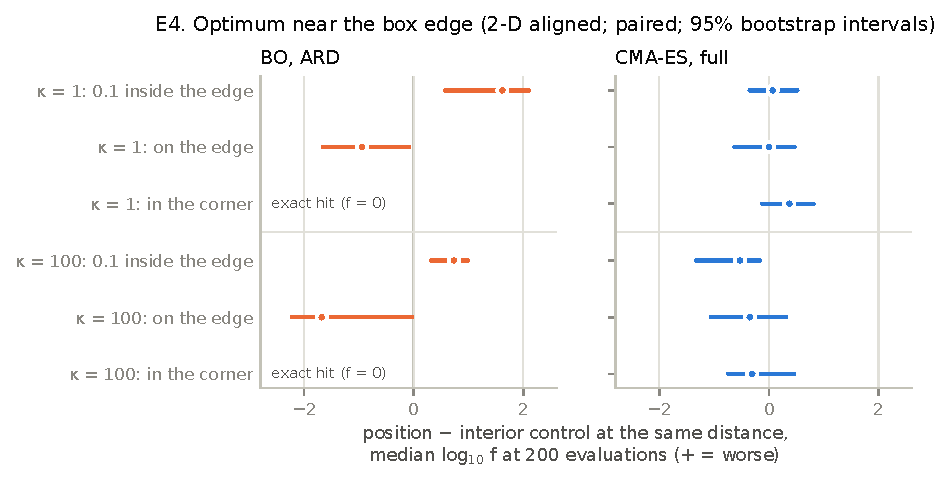
\includegraphics[width=0.66\linewidth]{figures/fig6_e4_boundary.pdf}
\caption{E4. Edge position minus a same-distance interior control (+ = worse).}
\label{fig:e4}
\end{figure}

%=====================================================================
\section{Beyond the quadratic}\label{sec:beyond}
%=====================================================================
\textbf{E5} (Fig.~\ref{fig:e5}). We wrote two predictions down before running.
\begin{itemize}
\item \emph{Rosenbrock (f8/f9).} \emph{Why this function:} every other problem here is a quadratic,
whose Hessian, and so whose orientation and conditioning, is the same everywhere. Rosenbrock is the
standard benchmark (COCO f8/f9) that is still unimodal and smooth, but whose valley floor \emph{bends}
along the parabola $z_2=z_1^2$ (Section~1). It changes one thing, the constancy of the geometry, and so
tests whether the explanation needs a \emph{local} tilt or only a global one. \emph{Why it needs a longer
budget:} a method must travel along the bending floor, and its learned orientation goes stale as the
floor turns. A step that is long along today's direction climbs the wall further on, so steps stay short
and the shape must be re-learned repeatedly. Near the optimum the valley is also narrow (local
$\kappa\approx2{,}500$). Full CMA-ES needs a median of about 500 evaluations to reach $10^{-5}$ (E9 below),
so 200 evaluations end before the final stage. \emph{At 200 evaluations (E5)} no method converges
($10^{-1.35}$--$10^{-0.49}$). Even ``aligned'' Rosenbrock has its valley at $63.5^\circ$ to the axes near the
optimum, so rotating it changes little. BO-full beats BO-ARD by 0.63 \ci{0.21}{1.08} (f8) and 0.39
\ci{-0.24}{0.96} (f9) decades, against 1.40 on the rotated quadratic, which is weak support for the
``one global tilt'' prediction only. \emph{With 4,000 evaluations (E9, CMA-ES only)} the picture is sharp.
Full CMA-ES reaches $10^{-5}$ in every run (median 535 and 492 evaluations), while diagonal CMA-ES reaches
it in 0\% of f8 runs and 27\% of f9 runs, about 3,500 evaluations behind (paired, failures counted at the
cap). We had predicted that both would converge. Diagonal fails even on the ``aligned'' f8, because what
matters is the valley's \emph{local} orientation, which is tilted near the optimum whatever the label says.
\item \emph{Noise} (additive, $\sigma\in\{0.01,1\}$; each method recommends its lowest observed point,
scored on the noise-free $f$, as the course brief requires). The prediction was that the noise fix would
backfire once the objective is noisy. It did not: fixed-noise BO still beat fitted-noise BO ($-0.41$
\ci{-0.73}{-0.10} at 200, $\sigma=0.01$). Noise removes CMA-ES's late lead (from $+1.35$ noise-free to
$+0.42$ and $-0.01$). It misleads CMA-ES's recommendation more than its search: at $\sigma=0.01$ it
evaluates points at $10^{-3.57}$ but recommends one at $10^{-2.40}$.
\end{itemize}

\begin{figure}[!htbp]
\centering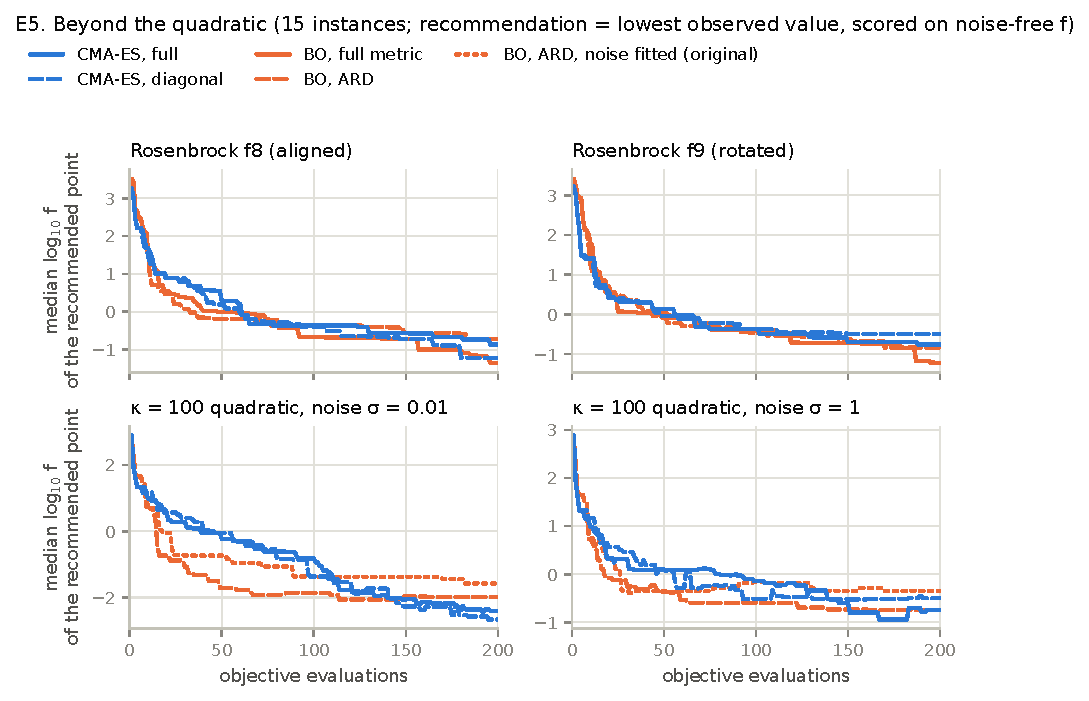
\includegraphics[width=0.80\linewidth]{figures/fig7_e5_other_functions.pdf}
\caption{E5. Median noise-free value of the recommended point. Dotted: BO-ARD with the noise fitted (original).}
\label{fig:e5}
\end{figure}

%=====================================================================
\section{Noisy evaluations: budget split and recommendation}\label{sec:noise}
%=====================================================================
\textbf{E6} (Fig.~\ref{fig:e6}) follows E5's noise test with the two questions the course brief poses.
How should a noisy budget be divided between new points and repeats, and which point should be
recommended? Setting: the aligned $\kappa=100$ quadratic, additive noise $\sigma\in\{0.01,0.1,1\}$, 200
noisy evaluations per run with repeats counted, and full CMA-ES and BO-ARD with the fix. Each
recommendation is scored on the noise-free $f$. The rules are R1, the lowest observed value; R2, the
model's estimate (CMA-ES's final mean, or the point with the lowest posterior mean of a GP refitted
\emph{with noise estimated}); and R3, the best average after re-evaluating the top five points.
\begin{itemize}
\item \emph{Rules.} For BO, R2 beats R1 by $0.30$ \ci{0.15}{0.78} decades at $\sigma=0.1$ and by $1.08$
\ci{0.28}{1.29} at $\sigma=1$: the search was fine, but picking the lowest reading threw it away. For
CMA-ES, the mean helps only with a larger population ($\lambda=24$: 0.47 and 0.33 decades, both
significant). With $\lambda=6$ it ties with R1, because a mean of three selected points averages little.
\item \emph{Splits.} Repeats did not pay at this budget. Resampling each CMA-ES candidate $4\times$
leaves 48 distinct points and costs 1.1--3.0 decades. BO replicates cost 1.6 and 1.1 decades at
$\sigma\le0.1$ and do not help at $\sigma=1$ ($+0.84$ \ci{-0.14}{1.68}), though they cut BO's computation
27-fold (5\,s against 141\,s). A final reserve of 40 re-evaluations never helped significantly. A
$4\times$ larger population, which averages without repeating, was the only split that helped (CMA-ES at
$\sigma=1$: $-0.57$ \ci{-0.85}{-0.08}), and it costs $+0.62$ at $\sigma=0.01$.
\item \emph{Across families.} With each family's best configuration, BO and CMA-ES are level at every
noise level ($+0.02$, $+0.08$, $-0.18$ decades; every interval contains 0). Three of our five written
predictions failed or held only in part (\texttt{code/run\_e6\_noise\_budget.py}).
\end{itemize}
At this budget the best use of noisy evaluations was to keep exploring new points and let a model
average at the end. One anomaly is unexplained: with replicates, BO's R2 is \emph{worse} than R1. A
plausible cause is that the averaged data are nearly noise-free, so the noise-fitting GP fails as in
Section~4.

\begin{figure}[!htbp]
\centering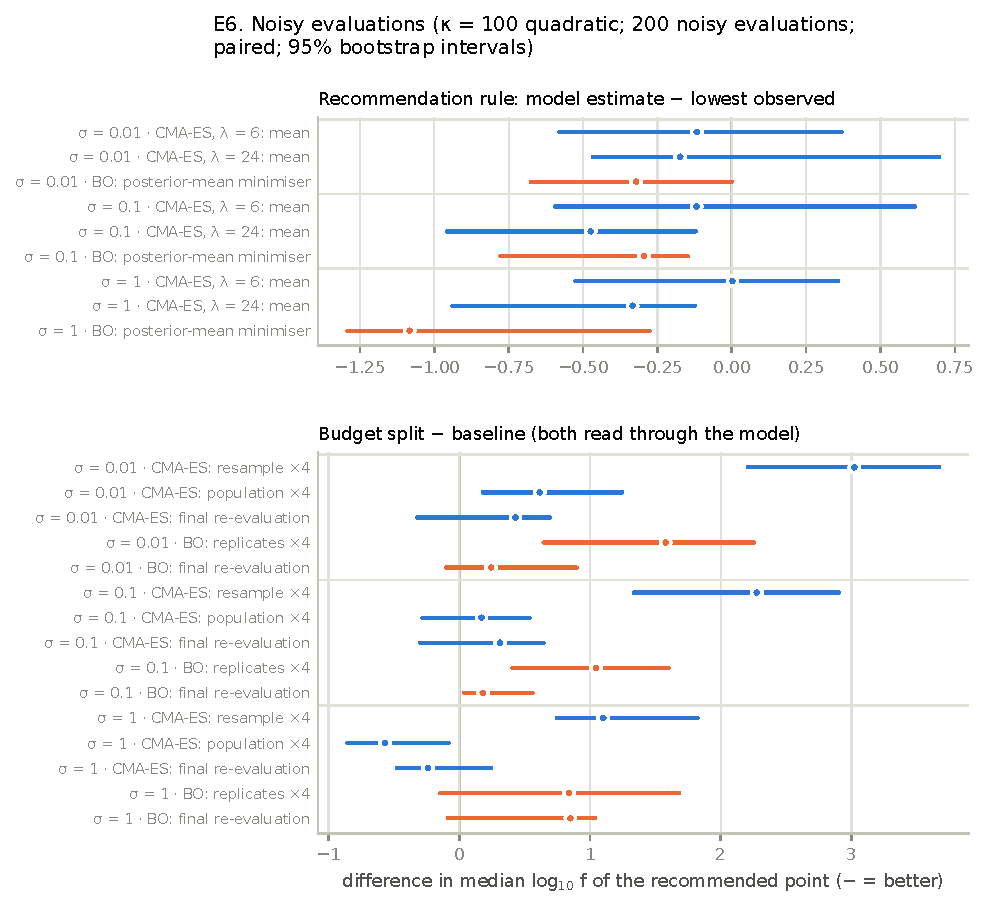
\includegraphics[width=0.66\linewidth]{figures/fig8_e6_noise.pdf}
\caption{E6. Top: model-based recommendation minus lowest reading on the same runs. Bottom: each budget
split minus the baseline. Negative = better.}
\label{fig:e6}
\end{figure}

%=====================================================================
\section{What is established, and what is not}
%=====================================================================
\textbf{Established.} (1) On rotated ill-conditioned quadratics, the axis restriction predicts failure
in both families: diagonal CMA-ES and ARD-BO pay, while their tilting counterparts do not, and the
penalty vanishes on aligned or well-conditioned problems. On the BO side this holds for two kernels, two
acquisition searches and a TuRBO-style trust region; on Rosenbrock, what matters is the local
orientation (E9). (2) Tilting has a modest cost when no tilt is
needed (up to $+21.6\%$ evaluations for CMA-ES; worse held-out RMSE for the full GP metric on aligned
problems). (3) CMA-ES's rank invariance survives the implementation exactly; its linear invariance holds
only under the stated condition on $C_0$. BO has neither invariance, and how $f$ is written can move it
by 1.7 decades. (4) The box is part of BO's model and invisible to CMA-ES; a fair comparison has to state
the bound handling for both. (5) Under noise at this budget, model-based recommendation (GP posterior
mean; a large-population CMA-ES mean) beats the lowest reading, and repeating evaluations does not pay.

\textbf{Uncertain or limited.} BO was run only in 2-D, so the dimension trend of the ARD penalty is inferred from CMA-ES (E1), not
measured. The cross-family comparison at 200 evaluations depends on BO's acquisition search: plain EI
stalls near $10^{-4}$, local candidates fix that but fall into a boundary trap, and trust-region BO is
strongest but shares the trap. No single BO configuration dominates. The full GP metric
is overconfident (worse log predictive density than ARD nearly everywhere), and about 2\% of fits still
miss the best hyperparameter optimum. CMA-ES ran without restarts. A check (E7) shows this does not matter here: full CMA-ES solves every
quadratic without them, and IPOP-style restarts (4 runs, population doubling from 6 to 48) leave diagonal
CMA-ES's rotated $\kappa=10^4$ failure in place (7\% reach $10^{-5}$ against 20\% for one long run),
because a restarted diagonal run still cannot tilt. Across machines, BO results agree in distribution but not run for run: re-running the original E2
elsewhere matched 40--93\% of BO-ARD runs and 0--27\% of BO-full runs to 0.01 decades, and one cell's
median moved by 0.6 decades. All before/after comparisons in the report are therefore paired on one
machine. With noise, the geometry argument predicts little at this budget. Several of our written predictions
failed or held only in part (E5, E6, E9) and are reported as such.

\textbf{For algorithm choice.} The question ``BO or CMA-ES?'' is partly the wrong one. Whether the
method can represent the problem's orientation matters as much as the family. A practitioner facing a
rotated, ill-conditioned problem should avoid an ARD kernel or a diagonal ES for the same reason. Under
noise, the choice of recommendation rule matters as much as the choice of family.

\small
\bibliographystyle{abbrvnat}
\bibliography{references}

\end{document}
